% =================================================================================================
% File:			gestione_amministrativa_della_revisione.tex
% Description:	Definisce la sezione relativa alla gestione amminitrativa della revisione
% Created:		2014/12/16
% Author:		Ceccon Lorenzo
% Email:		ceccon.lorenzo@mashup-unipd.it
% =================================================================================================
% Modification History:
% Version		Modifier Date		Change											Author
% 0.0.1 		2014/12/16 			iniziata stesura sezione gestione revisione	Lorenzo C.
% =================================================================================================
%

% CONTENUTO DEL CAPITOLO

\section{Gestione amministrativa della revisione}

	\subsection{Gestione delle anomalie e delle discrepanze}
	La fase di verifica porta alla ricerca di eventuali difetti, i quali possono essere errori logici oppure anomalie presenti nel codice. Il verificatore ha il compito di esaminare scrupolosamente il codice del prodotto e sottolineare le eventuali anomalie e problemi per essere risolti successivamente.
	
	\subsection{Procedure di controllo di qualità di processo}
	Il PDCA, noto anche come ciclo di Deming, è un metodo di gestione iterativo a quattro fasi per il controllo e il miglioramento continuo dei processi.\\
	Le quattro fasi che lo compongono sono:
		\begin{itemize}
			\item \textbf{Plan:} \textnormal{Stabilisce gli obiettivi e i processi necessari per ottenere risultati uguali a quelli attesi.}
			\item \textbf{Do:} \textnormal{Fase composta dall'attuazione del piano, dall'esecuzione del processo e dalla creazione del prodotto. Termina con una raccolta dei dati sul risultato di quanto ottenuto.}
			\item \textbf{Check:} \textnormal{Si confrontano i risultati ottenuti dalla fase precedente con i risultati attesi per verificare la presenza di differenze.}
			\item \textbf{Act:} \textnormal{Si effettuano correzioni laddove sono presenti differenze tra i risultati ottenuti e previsti. Si determinano le cause e dove applicare le modifiche per ottenere un miglioramento del processo e del prodotto.}
		\end{itemize}
		\begin{figure}[h]
			\centering
			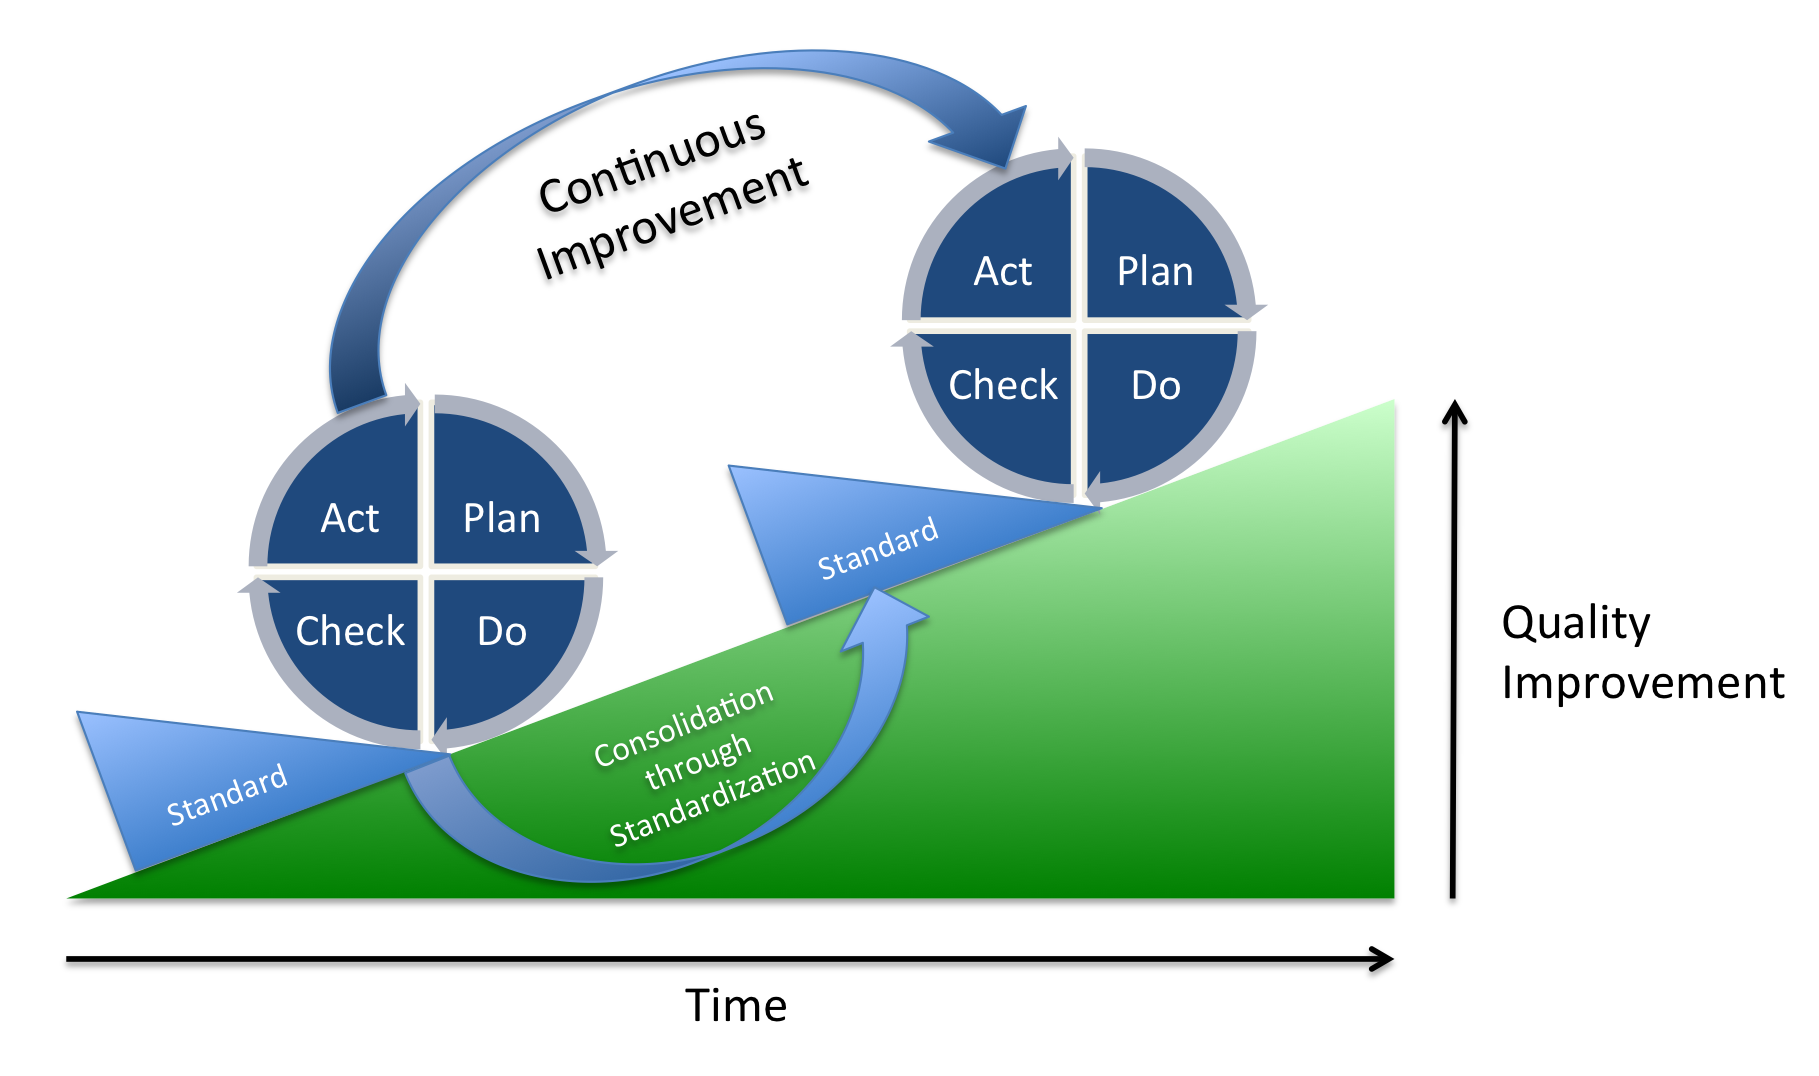
\includegraphics[width=90mm]{images/pdca.png}
			\caption{Ciclo di miglioramento della qualità PDCA}
		\end{figure}
	
	\subsection{Procedure di controllo di qualità di prodotto}
	
	
	\pagebreak